	\chapter{Topologický a měřitelný prostor}
	\section{Motivace k problematice stochastických systémů a procesů}
	Stochastické systémy a procesy vykazují náhodné chování, na rozdíl od systémů deterministických. U stochastických systémů tedy do budoucna nelze s absolutní přesností předpovídat chování takového systému.
	
	\begin{figure}
		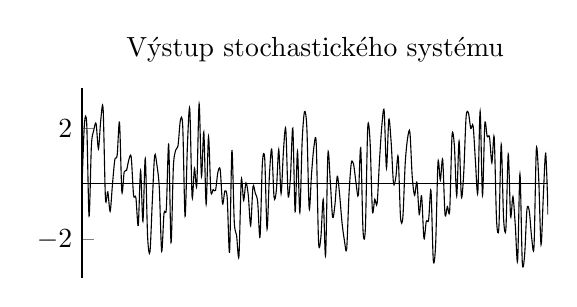
\begin{tikzpicture}[samples=200, domain=0:5*360]
	\begin{axis}[
        width=7.5cm, height=4cm,
        enlarge x limits=false,
        xtick=\empty,
        axis lines*=middle,
        title = Výstup stochastického systému
    ]
    \addplot [no markers, smooth] {sin(x)+rand*2};
    \end{axis}
\end{tikzpicture}
	\end{figure}
	
	\subsection{Doporučená literatura}
	\begin{enumerate}[noitemsep, label={[\arabic*]}]
	\item Havrda Jan; Stochastické procesy a teorie informace, ČVUT, 1985.
	\item Anděl Jiří; Stochastická analýza časových řad, SNTL, 1975.
	\item Prchal; Teorie pravděpodobnosti ve sdělovací technice, NADAS, 1975.
	\item Mandl Petr; Pravděpodobnostní dynamické modely, Academia, 1985.
	\item Papoulis A., Pilla S. U., Probability, Random Numbers and Stochastic Processes, Mc Graw Hill.
	\end{enumerate}
	
	\section{Základní pojmy}
	\subsubsection{Binární relace}
	Mějme proměnné $x,y$ a množiny $X,Y$, kde $x\in X$ a $y\in Y$. Binární relace je definována vztahem $R\subset X\times Y$, kde $R$ je relace a $X\times Y$ kartézský součin množin $X,Y$.
	
	\begin{note}{Příklad}
	Mějme množiny $X=\{a,b,c,d\}, Y=\{0,1,2\}$, pak je kartézský součin množina všech dvojic $(x,y)$, kde za $x$ lze dosadit prvek $a,b,c,d$ a za $y$ prvek $0,1$ nebo $2$.\br
	
	Relace $R$ je pak kterákoliv podmnožina množiny všech průsečíků, například těch vyznačených $\bullet$.
	
	\begin{figure}
		\input{TikZ/binrel.tikz}
	\end{figure}		
	\textbf{Závěr: } Relace je jistým zobecněním pojmu funkce.
	\end{note}
	
	\subsubsection{Zobrazení}
	Zobrazení $f$ množiny $X$ do množiny $Y$ je speciální lineární relace. Je to taková relace $f\subset X\times Y$, při které je ke každému prvku $x\in X$ přiřazen právě jeden prvek $y=f(x)\in Y$.\br
	
	Prvek $x$ je nazýván \textbf{vzorem} prvku $y$. Prvek $y$ je nazýván \textbf{obraz} prvku $x$. Množina $X$ se nazývá \textbf{definiční obor} zobrazení $f$. Množiny $Y$ se nazývá \textbf{obor hodnot}.
	
	\begin{note}{Příklad}
	Množiny $X,Y$ jsou stejné, jako v předchozím příkladu. Zobrazení $f$ je tedy například podmnožinou (označeno $\bullet$)
	\[ \left\{ (a,0), (b,0), (c,1), (d,2)\right\} \]
	
	\begin{figure}
		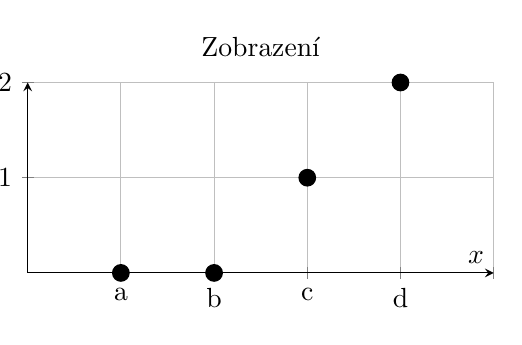
\begin{tikzpicture}[trim axis left, trim axis right]
		\begin{axis}[
		height=4cm,
		width = 7.5cm,
		title=Zobrazení,
		axis lines=middle,
		xlabel={$x$},
		ylabel={$y$},
		ylabel near ticks,
		ymin=0, ymax=2,
		xmin=0, xmax=5,
		ytick = {0,1,2},
		xtick = {},
		xticklabels = {0,0,a,b,c,d},
		grid = both
		]
		\addplot [only marks, mark size = 3] table {
		1 0
		2 0
		3 1
		4 2
		};
	\end{axis}
\end{tikzpicture}
	\end{figure}
	
	\textbf{Závěr: } Relace je jistým zobecněním pojmu funkce. Prvek $(b,1)$ na rozdíl od binární relace chybí, neboť by jinak k $b$ patřily dva obrazy!
	\end{note}
	
	\subsubsection{Obraz množiny}
	Množina takových $y=f(x)$, jejichž proměnná $y\in Y$ bude nabývat při změně hodnot $x\in A\subset X$, budeme označovat symbolem $f(A)$ a nazývat \textbf{obrazem množiny} $A$ při zobrazení $f$. Zřejmě platí:
	\[ f(A)=\big\{f(x): x\in A\big\}\subset Y \]
	
	Zobrazení $f$ množiny $X$ do množiny $Y$ se nazývá \textbf{zobrazením množiny} $X$ na množinu $Y$ právě tehdy, když ke každému prvku $y\in Y$ existuje takový prvek $x\in X$, že $y=f(x)$, tj. právě tehdy, když $f(x)=Y$.
	
	\subsubsection{Prosté zobrazení}
	Zobrazení $f$ množiny $X$ do množiny $Y$ se nazývá \textbf{prostým zobrazením}, právě když $f$ je zobrazením do množiny $Y$ a když pro každé dva různé prvky $x_1\in X$ a $x_2\in X$ platí
	\[ f(x_1)\neq f(x_2) \]
	
	Prosté zobrazení množiny $X$ na množinu $Y$ se též nazývá \textbf{vzájemně jednoznačné zobrazení} množiny $X$ na množinu $Y$.
	
	\subsubsection{Inverzní zobrazení}
	Je-li $f$ prosté zobrazení množiny $X$ na množinu $Y$, pak ke každému $y\in Y$ existuje právě jeden prvek $x\in X$ tak, že $f(x) = y$. Tím je definováno zobrazení $f^{-1}$ množiny $Y$ na množinu $X$. Toto zobrazení je prosté a nazývá se \textbf{inverzní zobrazení} k zobrazení $f$.
	
	\begin{note}{Příklad}
	Zobrazení všech přirozených čísel $\mathbb{N}$ do libovolné množiny $Y$ - například \textbf{posloupnost}. Zobrazení reálných čísel $\mathbb{R}$ do množiny reálných čísel $\mathbb{R}$ nazýváme reálnou funkcí (jedné) reálné proměnné.\br
	
	\textbf{Poznámka: } Zobrazení $f$ množiny $X$ do množiny $Y$ zapisujeme
	\[ f: X\to Y \]
	\end{note}
	
	\section{Prostory}
	\subsection{Topologický prostor}
	Budiž dána libovolná množina $X$ a soubor $\mathscr{T}$ jejich některých podmnožin $A$, kde $A\subset X$, pro který platí:
	\[ \begin{cases}\text{Je-li } A_i\in\mathscr{T} \text{ pro } i\in I\text{, kde $I$ je libovolná množina, pak také platí }\displaystyle\bigcup_{i\in I}A_i\in\mathscr{T} \\
	\text{Je-li } A_1,A_2\in\mathscr{T}\text{, pak také platí } A_1\cap A_2\in\mathscr{T}\\
	\text{Je-li } \emptyset\in\mathscr{T} \wedge x\in\mathscr{T}
	\end{cases}
	\]
	
	Pak dvojici $(X,\mathscr{T})$ nazveme \textbf{topologickým prostorem }, množinu $\mathscr{T}$ \textbf{topologií} na množině $X$ a prvky $A_i,A_i\in\mathscr{T}$ otevřenými množinami topologického prostoru $(X,\mathscr{T})$.
	
	\begin{note}{Poznámka}
	Ve fyzice a technice jsou důležitá tzv. spojitá zobrazení. Jsou to taková zobrazení, která blízká okolí každého bodu zobrazují na blízká okolí jeho obrazu.\br
	
	Předpokládejme, že je dán bod v rovině a je třeba určit polohu. V reálných podmínkách se to nikdy nepodaří přesně. Můžeme stanovit oblast $O_1$ a uvnitř té oblasti bod leží. Při jiných měřeních bychom dostali oblast $O_2$. Další oblast by byl průnik $O_1\cup O_2$.\br
	
	Nechť místo jednoho bodu je dána množina bodů. Sjednocení všech okolí tvoří okolí dané množiny. Okolí každé množiny budeme nazývat \textbf{otevřenou množinou}. Sjednocení libovolného souboru otevřených množin je otevřená množina. Průnik konečného (počtu) souboru otevřených množin je otevřená množina. 
	\end{note}
	
	\subsubsection{Okolí bodu}
	Okolím bodu $x\in X$ nazveme každou otevřenou množinu $A\in\mathscr{T}$, pro kterou platí $x\in A$. Jsou-li například $A_1$ a $A_2$  dvě okolí bodu $x\in X$ a platí-li $A_1\subset A_2$, pak je zřejmě $A_1$ bližším okolím bodu $x\in X$, než okolí $A_2$.\br
	
	Jelikož je dána otevřená množina $A,A\in\mathscr{T}$, pak doplněk této množiny se nazývá \textbf{uzavřená množina}. Množiny $\emptyset, X$ jsou tedy zároveň otevřené a uzavřené množiny topologického prostoru $(X,\mathscr{T})$.
	
	\subsubsection{Přirozená topologie}
	Nechť $X=\mathbb{R}$ a nechť $\mathscr{T}$ obsahuje libovolné sjednocení otevřených intervalů $(a,b)$, kde $a,b\in\mathbb{R}$. $\mathscr{T}$ je topologií na množině $\mathbb{R}$ a označuje se jako přirozená topologie množiny $\mathbb{R}$.
	
	\subsection{Spojité zobrazení topologického prostoru do jiného}
	Nechť jsou dány topologické prostory $(X,\mathscr{T}), (Y,U)$. Zobrazení $f: X\to Y$ topologického prostoru $(X,\mathscr{T})$ do topologického prostoru $(Y,U)$ nazveme spojitým, jestliže vzorem $A$ každé otevřené množiny $B\in U$, $A=f^{-1}(B)=\{x:f(x)\in B\}$ je množina otevřená. Jestliže tedy platí, že každé $B\in U$ je $f^{-1}(B)\in\mathscr{T}$.\br
	
	\subsubsection{Spojitost v bodě}
	Někdy je rozumné uvažovat spojitost zobrazení v bodě $x\in X$. Říkáme, že zobrazení $f: X\to Y$ je spojité v bodě $x_0\in X$, jestliže vzorem každého otevřeného okolí bodu $f(x_0)$ je nějaké (otevřené) okolí bodu $x_0$.
	
	\begin{note}{Poznámka}
	Je zřejmé, že zobrazení $f$ je spojité právě tehdy, je-li spojité v každém bodě.
	\end{note}
	
	\subsection{Měřitelný prostor}
	Teorie míry definuje problém nalezení délek různých křivek, ploch rovinných obrazců, objemů a hmotností těles, jako problém přiřazení reálných čísel souboru podmnožiny $X$, to jest jako problém nalezení zobrazení $\mu: \mathscr{U}\to\mathbb{R}$, $\mathscr{U}$ je soubor některých podmnožin základní množiny $X$, množina reálných čísel $\mathbb{R}$.\br
	
	Je pochopitelné, že má-li být zobrazení $\mu$ zobecněním pojmů délka, plocha, objem a hmotnost, musí mít následující vlastnosti:
	\begin{itemize}
		\item Je-li $A,B\in\mathscr{U}$, $A\subset B$, pak $\mu(A)\leq\mu(B)$. Tato vlastnost respektuje skutečnost, že velikost útvaru $A$ obsaženého v $B$ nesmí být větší, než velikost útvaru $A$.
		\item Je-li $A,B\in\mathscr{U}$, $A\cap B = \emptyset$, pak $\mu(A\cup B)=\mu(A)+\mu(B)$. Tato vlastnost respektuje skutečnost, že velikost útvaru složeného z nepřekrývajících se útvarů je rovna součtu jejich velikostí.
	\end{itemize}	
	
	\subsubsection{Elementární obrazce}
	Obrazce, které můžeme snadno změřit, mají fundamentální význam. Nazveme je elementárními obrazci $A$ a pro stručnost budeme soubor všech těchto obrazců označovat symbolem $\mathscr{S}$. Pro soubor elementárních obrazců platí:
	
	\begin{itemize}[noitemsep]
	\item $X$ je elementární obrazec, $x\in\mathscr{S}$
	\item Je-li $A$ elementárním obrazcem, je také elementární doplněk (označujeme $\bar{A}$) do množiny $X$ elementární obrazec, tj. jestliže $A\in\mathscr{S}\Rightarrow \bar{A}\in\mathscr{S}$.
	\item Jsou-li $A_1, A_2$ elementární obrazce, je také jejich disjunktní zobrazení elementárním obrazem.
	\item Jsou-li tedy $A_1,A_2\in\mathscr{S}, A_1\cap A_2=\emptyset A_1\cup A_2\in\mathscr{S}$. 
	\end{itemize}
	
	Konstruovat rovinné obrazce ve stále větším počtu, elementární prostory se mohou zmenšovat, dostat se k nějakému limitnímu případu (podobně pro objem), ...\br
	
	Podobně jako u rovinných obrazců můžeme postupovat při určování měr podmnožiny obecné množiny $X$. Dostaneme pak soubor $u$ podmnožin množiny $X$, pro který platí:
	\begin{itemize}[noitemsep]
	\item Množina $X\in \mathscr{U}$
	\item Je-li $A\in\mathscr{U}$, pak i elementární doplněk $\bar{A}\in\mathscr{U}$
	\item Je-li $A_i\in \mathscr{U}$ pro $i=1,2,\ldots$, pak též $\displaystyle\bigcup_{i=1}^\infty A_i\in\mathscr{U}$
	\end{itemize}
	
	Soubor $\mathscr{U}$ podmnožin množiny $X$ nazýváme \textbf{sigma algebrou} ($\sigma$-algebrou) na množině $X$ a jeho prvky \textbf{měřitelnými množinami}. Sigma ($\sigma$) označuje skutečnost, že do $\mathscr{U}$ patří vedle konečného také spočetné sjednocení prvků z $\mathscr{U}$. Uspořádané dvojice $(X, \mathscr{U})$ se nazývají \textbf{měřitelným prostorem} a uspořádaná trojice $(X,\mathscr{U},\mu)$ \textbf{prostorem s mírou}.\br
	
	Z vlastností $\sigma$-algebry plynou další vlastnosti:
	\begin{itemize}
		\item Platí $\emptyset\in \mathscr{U}$, poněvadž platí-li $x\in \mathscr{U}, \bar{x}\in \mathscr{U}$, jelikož $\bar{x}=\emptyset$, pak patří prázdná množina do $\sigma$-algebry.
		\item $A_1,A_2\in \mathscr{U} \Rightarrow A_1\cap A_2\in \mathscr{U}$, neboť $\bar{A}_1, \bar{A}_2\in \mathscr{U}, \bar{A}_1\cup\bar{A}_2\in \mathscr{U}$ a $\overline{\overline{A}_1\cup\overline{A}_2}\in \mathscr{U}$, podle Morganova pravidla $\overline{\overline{A}_1\cup\overline{A}_2} = A_1\cap A_2$ a tedy $A_1\cap A_2\in \mathscr{U}$.
		\item $\mu(\emptyset)=0$, neboť $\emptyset\in \mathscr{U}$ a pro libovolné $A\in \mathscr{U}$ platí $A\cap\emptyset = \emptyset$, pak $\mu(A\cup \emptyset)=\mu(A)+\mu(\emptyset)=\mu(A)$, jelikož $A\cup \emptyset = A$.
		\item Rovněž platí $0\leq A$, neboť $A,\emptyset\in \mathscr{U}, \emptyset\subset A$ a $\mu(\emptyset)\leq\mu(A)$ a protože platí $\mu(\emptyset)=0$, pak je úvodní tvrzení \textbf{pravdivé}.
	\end{itemize}
	
	\begin{note}{Příklad}
	Jednoduchým příkladem míry je aritmetická míra, která každé podmnožině množiny $X$ přiřazuje míru, jež je rovna počtu prvků dané podmnožiny.
	\end{note}
	
	\begin{note}{Příklad}
	Diracova míra každé podmnožině $A$ množiny $X, A\subset X$, přiřazuje míru: 
	
	\[ \mu(A) = \begin{cases} 1& \text{jestliže } x_0\in A\\ 0 & \text{jestliže } x_0\not\in A\text{, kde $x_0$ je pevně zvolený bod}  \end{cases} \]
	\end{note}
	
	\begin{note}{Příklad}
	Lebesquerova míra přiřazuje v $\mathbb{R}^1$ každému intervalu délku, v $\mathbb{R}^2$ každému obdélníku obsah a v $\mathbb{R}^n$, kde $n=3,4,\ldots, m$ každému n-rozměrnému kvádru jeho n-rozměrný objem.
	\end{note}
	
	\subsection{Měřitelné zobrazení}
	Nechť $(X,\mathscr{U})$ je měřitelný prostor, $(Y,\mathscr{T})$ topologický prostor a $f:X\to Y$ zobrazení. Pak říkáme, že $f$ je \textbf{měřitelné zobrazení} právě tehdy, když pro každou otevřenou množinu $B\in\mathscr{T}$ je $f^{-1}(B)$ měřitelnou množinou, tj. když platí
	\[ f^{-1}(B)=\big\{ x:f(x)\in B\in\mathscr{T}\big\}\in \mathscr{U} \]
	
	\subsubsection{Borelovská $\sigma$-algebra}
	Nechť je dán topologický prostor $(Y,\mathscr{T})$. Pak sigma algebra podmnožin množiny $Y$, generované souborem prvků množiny $\mathscr{T}$ se nazývá \textbf{borelovská $\sigma$-algebra}, značí se často symbolem $\mathscr{B}$ a její prvky se nazývají \textbf{borelovskou množinou} na topologickém prostoru $(Y,\mathscr{T})$. Borelovskými množinami topologického prostoru $(Y,\mathscr{T})$ jsou tedy všechny množiny otevřené, všechny jejich doplňky, tj. všechny množiny uzavřené, všechna společná sjednocení otevřených a uzavřených množin. Dvojice $(Y,B)$ je měřitelný prostor.\br
	
	Nechť je dán měřitelný prostor $(X,\mathscr{U})$, topologický prostor $(Y,\mathscr{T})$ a zobrazení $f:X\to Y$ a nechť symbol $\mathscr{S}$ označuje soubor všech podmnožin $S$ množiny $Y$, pro kterou platí:
	
	\[ f^{-1}(S)\in \mathscr{U}\text{, potom } X=f^{-1}(Y)\in \mathscr{U} \Rightarrow Y\in \mathscr{U} \]
	
	Patří-li $S$ do množiny $\mathscr{S}$, tj. $S\in\mathscr{S}$, pak zobrazení $f^{-1}(S)\in \mathscr{U}$ a $f^{-1}(S)\in \mathscr{U}, f^{-1}(S) = f^{-1}(\bar{S})\in \mathscr{U}$, pak také $\bar{S}\in\mathscr{S}$.\br
	
	Je-li $S_i\in\mathscr{S}, i=1,2,\ldots,m$, pak platí
	\[ f^{-1}(S_i)\in \mathscr{U} \Rightarrow \bigcup_{i=1}^\infty f^{-1}(S_i) = f^{-1}\left(\bigcup_{i=1}^\infty S_i\right)\in \mathscr{U} \Rightarrow \bigcup_{i=1}^\infty S_i\in\mathscr{S} \]
	
	Soubor $\mathscr{S}$ je tedy dle definice $\sigma$-algebrou podmnožin množiny $Y$. Bude-li nyní zobrazení $f$ měřitelné, obsahuje dle definice měřitelnosti množiny $\mathscr{S}$ všechny otevřené množiny na topologickém prostoru $(Y,\mathscr{T})$ a protože je $\mathscr{S}$ $\sigma$-algebrou, obsahuje též všechny množiny \textbf{borelovské}.\br
	
	Je-li tedy $f$ měřitelné zobrazení měřitelného prostoru $(X,\mathscr{U})$ do topologického prostoru $(Y,\mathscr{T})$,  pak vzor $f^{-1}(B)$ každé borelovské množiny $B\in\mathscr{B}$ na $(Y,\mathscr{T})$ patří do $\sigma$-algebry měřitelných množin $\mathscr{U}$. Toto tvrzení je důležité pro základní teorii pravděpodobnosti.